% https://stackoverflow.com/a/71338316
\documentclass{beamer}

\usepackage{tikz}
\usetikzlibrary{arrows}
\usetikzlibrary{tikzmark}


\begin{document}
    
\begin{frame}
\begin{columns}
\begin{column}{0.5\textwidth}
\centering
  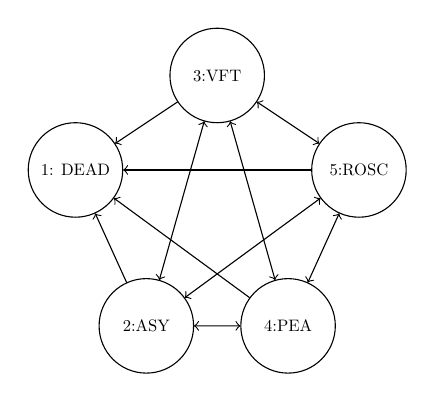
\begin{tikzpicture}[scale=0.6,transform shape,every state/.style={minimum width={2cm} ,thick,align=center},state/.style={circle, draw, minimum size=2cm}]
  \node[state] (1) {1: DEAD};
  \node[state] at (3, 2) (3) {3:VFT};
  \node[state] at (6, 0) (5) {5:ROSC};
  \node[state] at (1.5, -3.3) (2) {2:ASY};
  \node[state] at (4.5, -3.3) (4) {4:PEA};
  
  \draw[<-] (1) -- node [midway,above] {} (2);
  \draw[<-] (1) -- node [midway,below] {} (3);
  \draw[<-] (1) -- node [midway,below] {} (4);
  \draw[<-] (1) -- node [midway,below] {} (5);
  
  \draw[<->] (2) -- node [midway,below] {} (3);
  \draw[<->] (2) -- node [midway,below] {} (4);
  \draw[<->] (2) -- node [midway,below] {} (5);
  
  \draw[<->] (3) -- node [midway,below] {} (4);
  \draw[<->] (3) -- node [midway,below] {} (5);
  
  \draw[<->] (4) -- node [midway,below] {} (5);
  \end{tikzpicture}
\end{column}

\begin{column}{.1\textwidth}
\tikz\draw[blue,->] (0,0) -- (\textwidth,0);
\end{column}

\begin{column}{0.4\textwidth}
\centering
    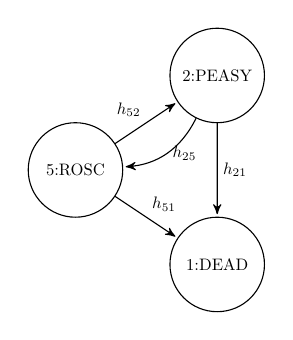
\begin{tikzpicture}[scale=0.6,transform shape, >=stealth', shorten >=1pt, auto, scale=1, 
    transform shape, align=center, 
    state/.style={circle, draw, minimum size=2cm}]

    \node[state] at (0,0) (5) {5:ROSC};  
    \node[state] at (3,-2) (1) {1:DEAD};
    \node[state] at (3,2) (2) {2:PEASY};

    \path[->] (5) edge node {$h_{51}$} (1)
              (5) edge node {$h_{52}$} (2)
              (2) edge node {$h_{21}$} (1)
              (2) edge [bend left] node [right] {$h_{25}$} (5);

    \end{tikzpicture}
\end{column}
\end{columns}

\end{frame} 
    
\end{document}
